\documentclass[preprint]{elsarticle}
\usepackage[latin1]{inputenc}
\usepackage[english]{babel}
%\usepackage[T1]{fontenc}
%\usepackage{textcomp}
\usepackage{graphicx}
\usepackage{color}
%\usepackage{setspace}
\usepackage{url}

\begin{document}

\begin{frontmatter}

%%%%%%%%%%%%%%%%%%%%%%%%%%%%%%%   TITLE   %%%%%%%%%%%%%%%%%%%%%%%%%%%%%%%

\title{Mobility analysis in a Smart City}
% Antonio - Esto es por poner algo, hay que cambiarlo, claro

%%%%%%%%%%%%%%%%%%%%%%%%%%%%%%%   AUTHORS   %%%%%%%%%%%%%%%%%%%%%%%%%%%%%%%

\author{author1, author2, author3, author4}
\ead{\{author1, author2, author3, author4\}@ugr.es}
\address{Departamento de Arquitectura y Tecnolog�a de Computadores.\\ ETSIIT - CITIC. University of Granada, Spain}

%\maketitle

%
%%%%%%%%%%%%%%%%%%%%%%%%%%%%%%%%%   ABSTRACT   %%%%%%%%%%%%%%%%%%%%%%%%%%%%%%%%%
%
\begin{abstract} 
The wonderful abstract
\end{abstract}

%
%%%%%%%%%%%%%%%%%%%%%%%%%%%%%%%%%   KEYWORDS   %%%%%%%%%%%%%%%%%%%%%%%%%%%%%%%%%
%
\begin{keyword}
Smart traffic \sep Transit indicators \sep Traffic forecast \sep Mobility analysis
\end{keyword}
% Antonio - A a�adir y mejorar

\end{frontmatter}


%-------------------------------------------------------------------------------
%%%%%%%%%%%%%%%%%%%%%%%%%%%%%%%   INTRODUCTION   %%%%%%%%%%%%%%%%%%%%%%%%%%%%%%%
%-------------------------------------------------------------------------------

\section{Introduction}
\label{sec:intro}

Nowadays, any system that collect reliable traffic information which is useful for wide population must be in mind for the society because the information increases the ability of improvement of any community. The information in our society is power and everybody tries to get it from any trustworthy source. Moreover, if this information is not available using any other previous commercial system, the innovation, the improvement and the success is guaranteed.

Traffic information is currently gathered using several kind of devices. The local, regional or national governments use these data aiming for improvements in the maintenance of roads and services, for computing useful traffic statistics, or to optimize the traffic light synchronization, among other uses. This information is considered in several ways, from improving the traffic flow inside the city to the end-users, drivers, who can profit by optimally planning their trips according to the current, or future, status of the traffic flow. Thus, gathered traffic information must be reliable and useful both, in real time and also in the near future, by means of forecasting tools, for instance.

The traffic monitors nowadays include pneumatic tubes, loop detectors, floating vehicles or automatic Optical Character Recognition (OCR) among others, but most of them are not able to identify and follow the same vehicle along the road network. In this paper we present a system able to do this while improving the quality of the gathered information and allowing the easy construction of traffic flow models or mobility graphs. In addition, the proposed system is formed by low-cost devices, which is another advantage over the usual monitoring systems, since the cost is an important factor for authorities which tend to install the simplest and cheapest monitors.

Each device, called MOBYWIT (Mobility by Wireless Tracking), evolution of the system presented in \cite{castillo2014_book_sipesca}, is based in a single-board computer which monitors the radioelectric space catching Bluetooth (BT) and WiFi signals emitted by other devices. These will be mainly smartphones or hands-free systems on vehicles, which are detected and identified by means of their Media Access Control number (MAC) - which is unique - and stored as a traffic `step'. Thus, depending on the position of the monitoring device, we could gather information about specific people or vehicles displacements. In order to respect the person's privacy and data protection laws, the MAC is one-direction encrypted before storing it, so, we cannot relate a captured MAC with any person.

These devices cannot detect all the real persons and vehicles moving close to them, since not all of them will be emitting BT or WiFi signals, but after a poll that we did among 600 people we can conclude that we detect around the 22\% of the drivers due to BT detection and around the 70\% of the drivers due to WiFi detection, which are good figures to be considered as representative of the real traffic flows.

In this paper we present, in addition to the monitoring system \textit{MOBYWIT}, three different scenarios in which real traffic/mobility data has been gathered. They are namely: a Spanish highway with six different nodes (devices) and two main roads, a junction inside the city of Granada and a discotheque. These data have been deeply processed, extracting interesting models such as in/out matrices and flow graphs that had been exhaustively analyzed. Moreover, some forecast techniques have been applied on them, in order to predict the traffic/movements inside those scenarios in a near future.

The rest of the work is structured as follows...


%----------------------------------------------------------------------------
%%%%%%%%%%%%%%%%%%%%%%%%%%%%%   STATE OF THE ART  %%%%%%%%%%%%%%%%%%%%%%%%%%%
%----------------------------------------------------------------------------


\section{Background and state of the art}
\label{sec:preliminaryconcepts}

- Talk about current technologies of monitoring (a couple of paragraphs)\\
- Talk about traffic modeling and forecast or other analyses on it.\\


%------------------------------------------------------------------------------
%%%%%%%%%%%%%%%%%%%%%%%%%%%%%%%%%%  MOBYWIT  %%%%%%%%%%%%%%%%%%%%%%%%%%%%%%%%%%
%------------------------------------------------------------------------------

\section{MOBYWIT}
\label{sec:mobywit}

This device was designed by one of the authors and it is based in a single-board computer, Raspberri Pi\footnote{https://es.wikipedia.org/wiki/Raspberry\_Pi}. It has two USB cards, namely a Bluetooth (BT) and WiFi ones, and it uses their interfaces in monitor mode, scanning the radioelectric space searching for BT devices and beacon frames (for WiFi).

Every device, called MOBYWIT (***from Mobility...***) is formed by a hardware and a software layer very interconnected. It is part in the whole monitoring system, which also includes Cloud-based storage and computing services. The software architecture of the whole system is shown in Figure \ref{fig:mobywit}.

\begin{figure}[ht]
	\begin{center}
		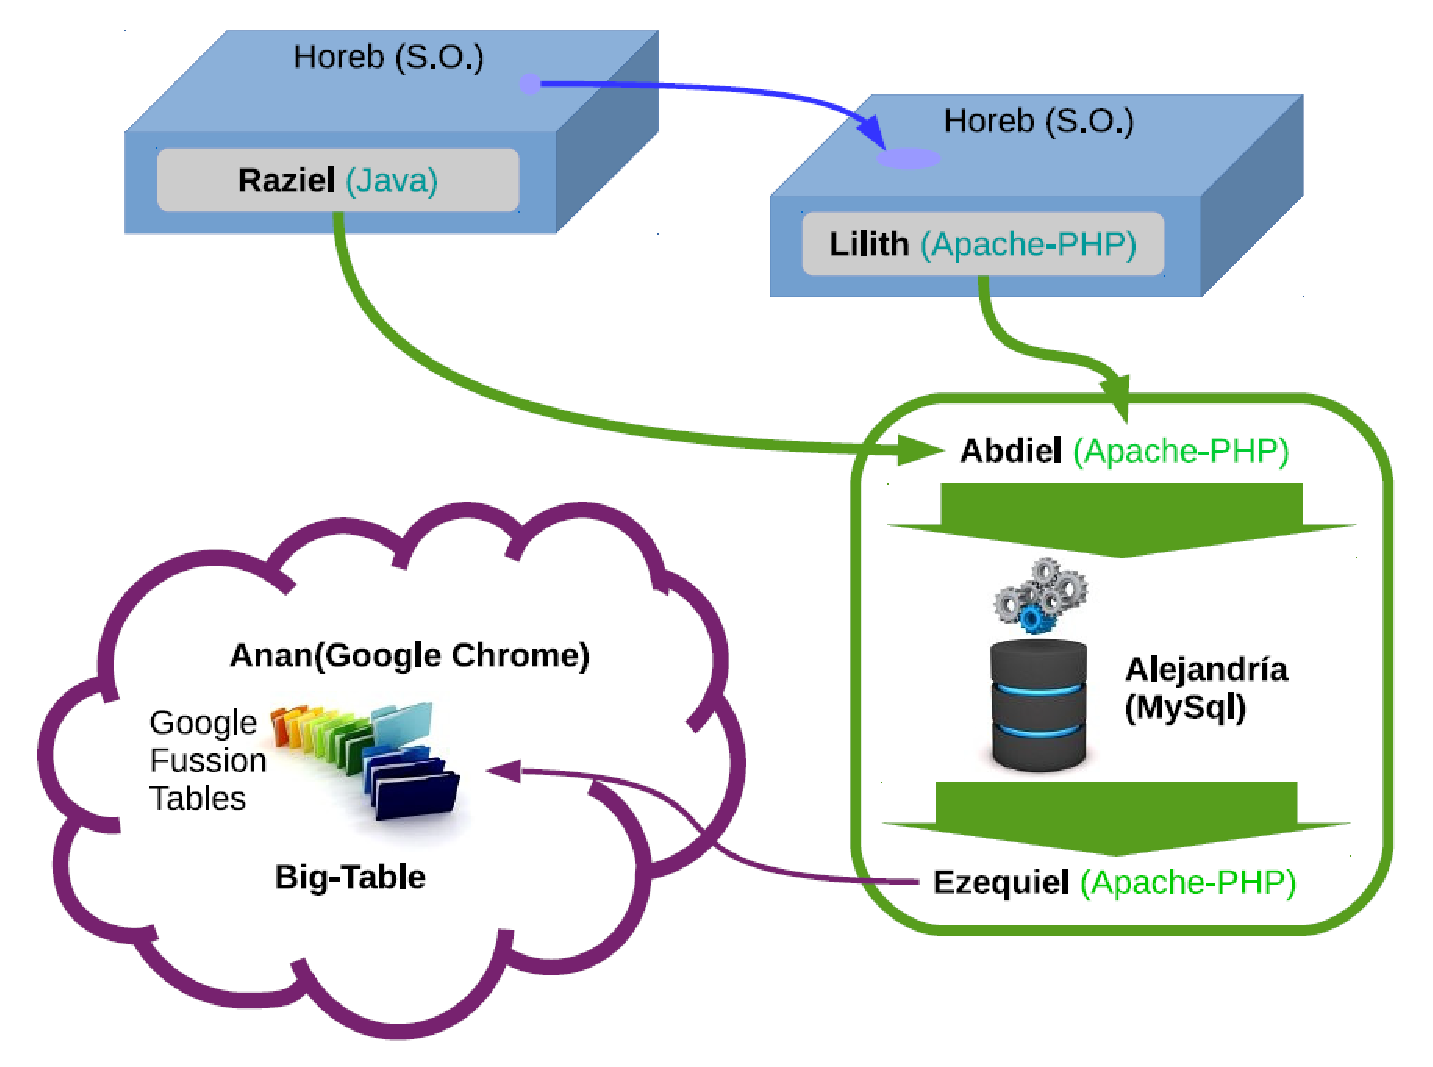
\includegraphics[scale=0.4]{imgs/mobywit.eps}
		\caption{Monitoring system architecture}
	\label{fig:mobywit}
	\end{center}
\end{figure}

As it can be seen in that figure, there are six main parts in the software layer of the system, which are unidirectionally connected by a strict data flow. They are have been named as:
\begin{itemize}

\item \textit{Raziel}: This module is in charge of the detections of BT and WiFi devices as well as of their identification (extracting and encrypting the MAC) and the periodic submission of this information to the server. It is run in the device and implemented in Java.

\item \textit{Lilith}: This module acts as a gateway between the network of devices and the server. It allows the communications between nodes and between them and external networks. This component is also run in every device and implemented in PHP.

\item \textit{Abdiel}: This component implements a set of services for accessing the devices from 'outside' (mainly for activate/deactivate or update them). In addition it performs the storage of gathered data (in blocks) in the server database. It is also implemented in PHP.

\item \textit{Alejandr�a}: This is the database of the system. It is a MySQL instance placed in a local server. It is optimized (using indexes and table partitioning) to provide a close to real-time processing and data service.
Ezequiel: This module is responsible of the publication of data in a cloud-based storage. It includes data mining, machine learning and forecast techniques to process these data in order to publish interesting or useful information about them.

\item \textit{Anan}: This is the cloud-based storage and services. It is based in Google technology so Anan stores and manages the data in a NoSQL format, by means of Google Fusion Tables. It also offers advanced visualization methods to be more usable and attractive for the end-user of the system.

\end{itemize}

In addition, and as it is shown in Figure 1, the device runs an specific Operative System, called \textit{Horeb}, which is a modification of the original Raspbian 3.10.24, adapted by MOBYWIT system designer to be more robust (to power fails, for instance) and reliable.

%----------------------------------------------------------------------------
%%%%%%%%%%%%%%%%%%%%%%%%%%%   TRAFFIC in a HIGHWAY  %%%%%%%%%%%%%%%%%%%%%%%%%
%----------------------------------------------------------------------------

\section{Analysis of the traffic in a highway}
\label{sec:traffic}

Study of the traffic with data from the DGT nodes...

%----------------------------------------------------------------------------
%%%%%%%%%%%%%%%%%%%%%%%%%%%%   TRAFFIC in a CITY  %%%%%%%%%%%%%%%%%%%%%%%%%%%%
%----------------------------------------------------------------------------

\section{Analysis of the traffic in a city}
\label{sec:city}

Study of the traffic with data from the Granada nodes...

%----------------------------------------------------------------------------
%%%%%%%%%%%%%%%%%%%%%%%%%%%   PELOPLE'S MOBILITY  %%%%%%%%%%%%%%%%%%%%%%%%%%%
%----------------------------------------------------------------------------

\section{Analysis of people's mobility in a building}
\label{sec:mobility}

Study of the traffic with data from the ETSIIT/Discoteque nodes...

%----------------------------------------------------------------------------
%%%%%%%%%%%%%%%%%%%%%%%%%%%%%%%   CONCLUSIONS  %%%%%%%%%%%%%%%%%%%%%%%%%%%%%%%
%----------------------------------------------------------------------------

\section{Conclusions}
\label{sec:conclusions}

In this work, we have done several things...

%%%%%%%%%%%%%%%%%%%%%%%%%%%%%  ACKNOWLEDGEMENTS %%%%%%%%%%%%%%%%%%%%%%%%%%%%%%%%

\section{Acknowledgements}
This paper has been funded in part by...

\bibliographystyle{elsarticle-num}
\bibliography{mobility}

\end{document}
